%The implementation covers some of the implementation details of your project.
%This is not intended to be a low-level description of every line of code that
%you wrote but covers the implementation aspects of the projects.

%This section is usually 3-5 pages.

\section{Framework overview}

\subsection{API requirements} \label{implementation:api-requirements}

The main requirement for developing the uncertainty quantification package is the \textit{scikit-learn} compatibility which imposes constraints on how the models are created, trained and evaluated. In particular, all models should implement the \textit{fit} and \textit{predict} functions as well as \textit{predict\_proba} for classification models. To ensure full compatibility with the \textit{scikit-learn} library (e.g. grid search, etc.), several other development guidelines should be followed, such as the instantiation rule: "every keyword argument accepted by \textit{\_\_init\_\_} should correspond to an attribute on the instance.". Such guidelines are made available to \textit{scikit-learn} contributors at this \href{https://scikit-learn.org/dev/developers/develop.html}{link} and were taken into consideration during the development phase. 

% explain target API return_std
In the context of uncertainty quantification, a few regression models capable of deriving uncertainty scores are already available in the \textit{scikit-learn} API: \href{https://scikit-learn.org/stable/modules/generated/sklearn.gaussian_process.GaussianProcessRegressor.html#sklearn.gaussian_process.GaussianProcessRegressor}{Gaussian Process regressor}, \href{https://scikit-learn.org/stable/modules/generated/sklearn.linear_model.BayesianRidge.html#sklearn.linear_model.BayesianRidge}{Bayesian Ridge regressor} and \href{https://scikit-learn.org/stable/modules/generated/sklearn.linear_model.ARDRegression.html#sklearn.linear_model.ARDRegression}{Automatic Relevance Determination regressor (ARD)}. The UQ API chosen by these models is articulated around the \textit{predict} function:


\begin{lstlisting}[language=Python, caption=UQ sklearn API.]
    mean_pred, std_pred = model.predict(X, return_std=True)
\end{lstlisting}

A default parameter \textit{return\_std} is added to the prediction function. If set to true, the function returns a tuple of arrays: the mean predictions and their standard deviations. This API is extended to all predictors, i.e. classifiers and regressors in the package. To make a clear distinction between data and model uncertainty, the following syntax is adopted: 

\begin{lstlisting}[language=Python, caption=Extraction of uncertainty scores from predictions.]
    # Task 1: data UQ regression
    uq_preds = data_uq_regressor.predict(X, return_std=True)
    preds, std = uq_preds[:, 0], uq_preds[:, 1]
    # Task 2: data UQ classification
    uq_preds = data_uq_clf.predict(X, return_std=True)
    preds, entropy = uq_preds[:, 0], uq_preds[:, 1]
    # Task 3: model UQ estimator (regression or classification)
    preds, std = model_uq.predict(X, return_std=True)
\end{lstlisting}

The output of a data UQ model is a 2D array containing the mean predictions in the first column and the uncertainty scores in the second. Model UQ predictions are tuples as defined in scikit-learn. Furthermore, several utility functions are made available to the users to produce confidence internals, conformal predictions, calibration, uncertainty plots, etc.

\subsection{Architecture}

The package is organised as a set of predictor wrappers which all take a base predictor as the main argument and return an updated predictor following the API requirements defined in section \ref{implementation:api-requirements}. %An overview of the data uncertainty regressor and classifier wrappers is shown in figure \ref{fig:diagram-data-uq-wrappers}. 
Calibration, model UQ and data UQ wrappers are meant to be chained one on top of the others as highlighted in figure \ref{fig:diagram-uq-wrappers} and code below. The \textit{fit} method only needs to be called on the top-level wrapper to train all subsequent ones. 
A hierarchy of the different classes implemented in the package is shared in figure \ref{fig:class-hierarchy}. 

\begin{lstlisting}[language=Python, caption=Extraction of uncertainty scores from predictions.]
    uq_model = CalibratedRegressorCV(
        ModelUQWrapper(DataUQWrapper(base_estimator))
    ).fit(X_train, y_train)
    preds, std = uq_model.predict(X_test, return_std=True)
\end{lstlisting}


%Sklearn abstract class & Base estimator                         & BaseEnsemble
%UQlearn abstract class & PredictWrapper                         & BaseEnsembleUQ
%UQlearn base class     & RegressorWrapper & ClassifierWrapper   & EnsembleUQRgressorWrapper & EnsembleUQClassifierWrapper
%UQlearn specifics      & QuantileRegressor & BayesianRgressorWrapper  & CatBoostRegressorWrapper & EnsembleRegressorWrapper & AdversarialClassifier & % BaggingUQRegressor & BaggingUQClassifier & AdversarialEnsembleUQClassifier 





\begin{figure}[h!]
    \centering
    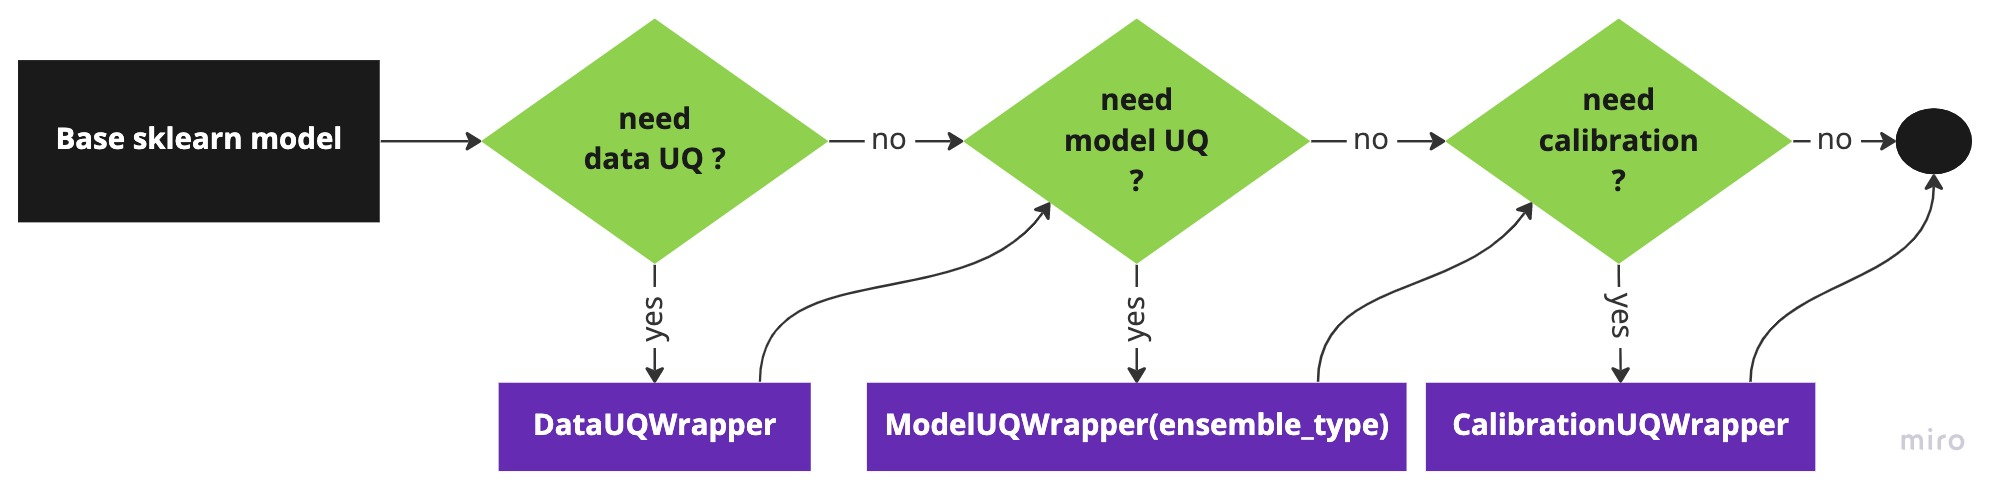
\includegraphics[width=.8\linewidth]{figures/implementation/diagram-sequence-wrappers.jpg}
    \caption{Schematic view of UQ wrappers and how they are built one on the other.}
    \label{fig:diagram-uq-wrappers}
\end{figure}

%\begin{figure}[htbp]
%    \centering
%    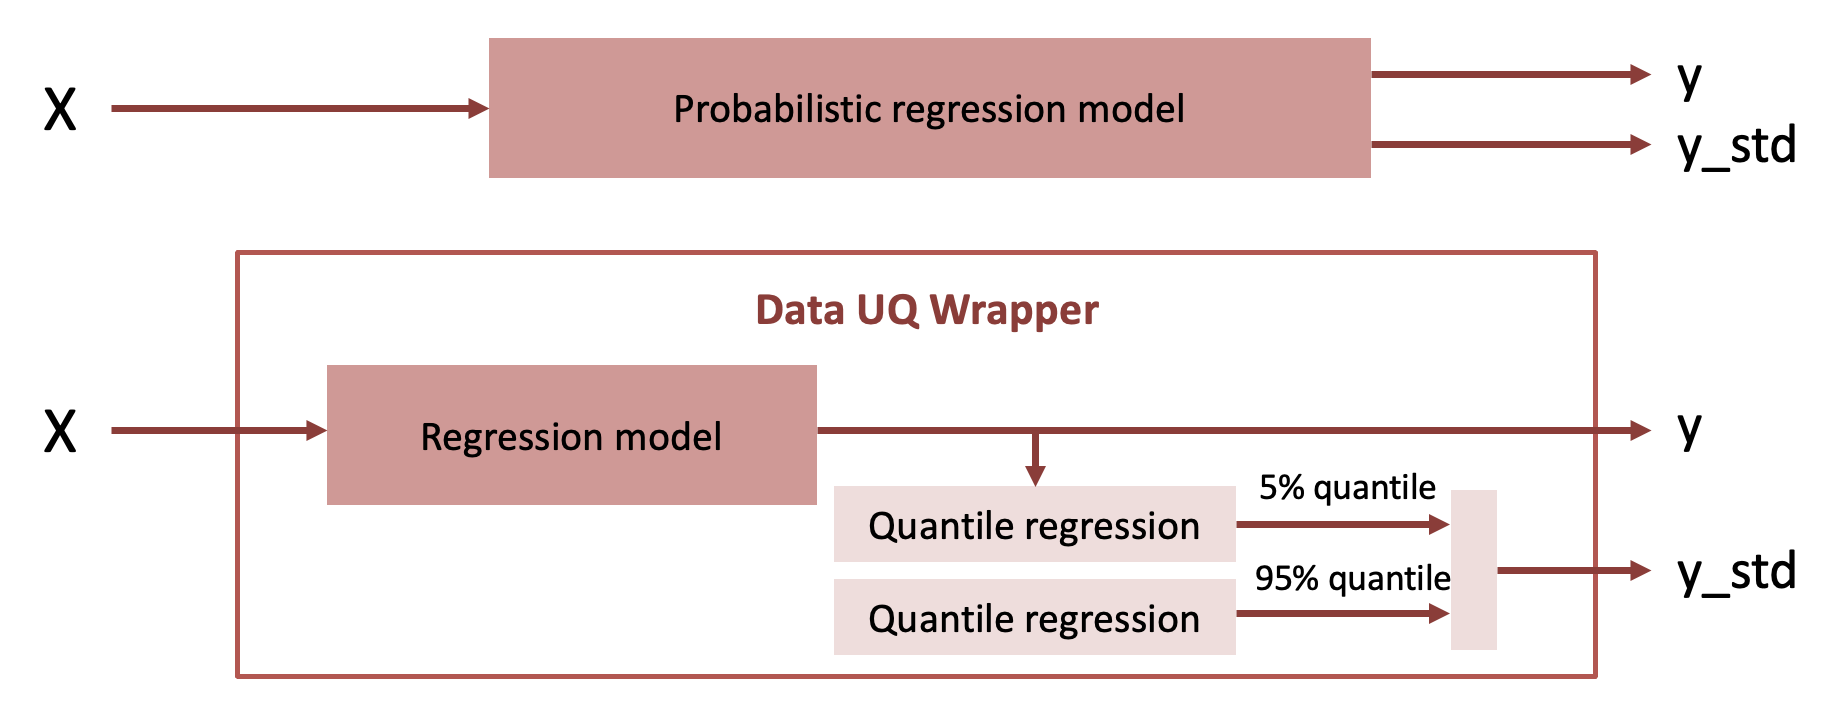
\includegraphics[width=.6\linewidth]{figures/implementation/diagram-uq-regressor.png}
%    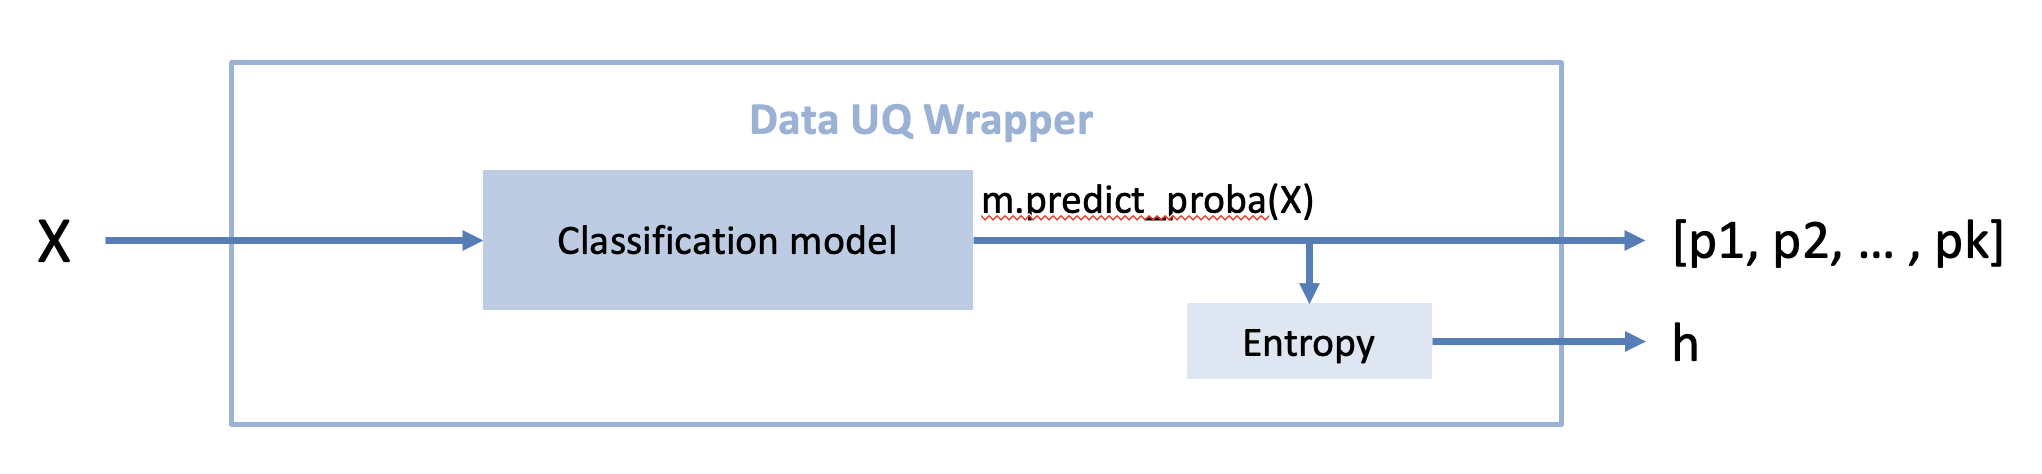
\includegraphics[width=.6\linewidth]{figures/implementation/diagram-uq-classifier.png}
%    \caption{Schematic view of data UQ wrappers (classification and regression).}
%    \label{fig:diagram-data-uq-wrappers}
%\end{figure}

\begin{figure}[htbp]
     \centering
     \begin{subfigure}[b]{0.32\textwidth}
         \centering
         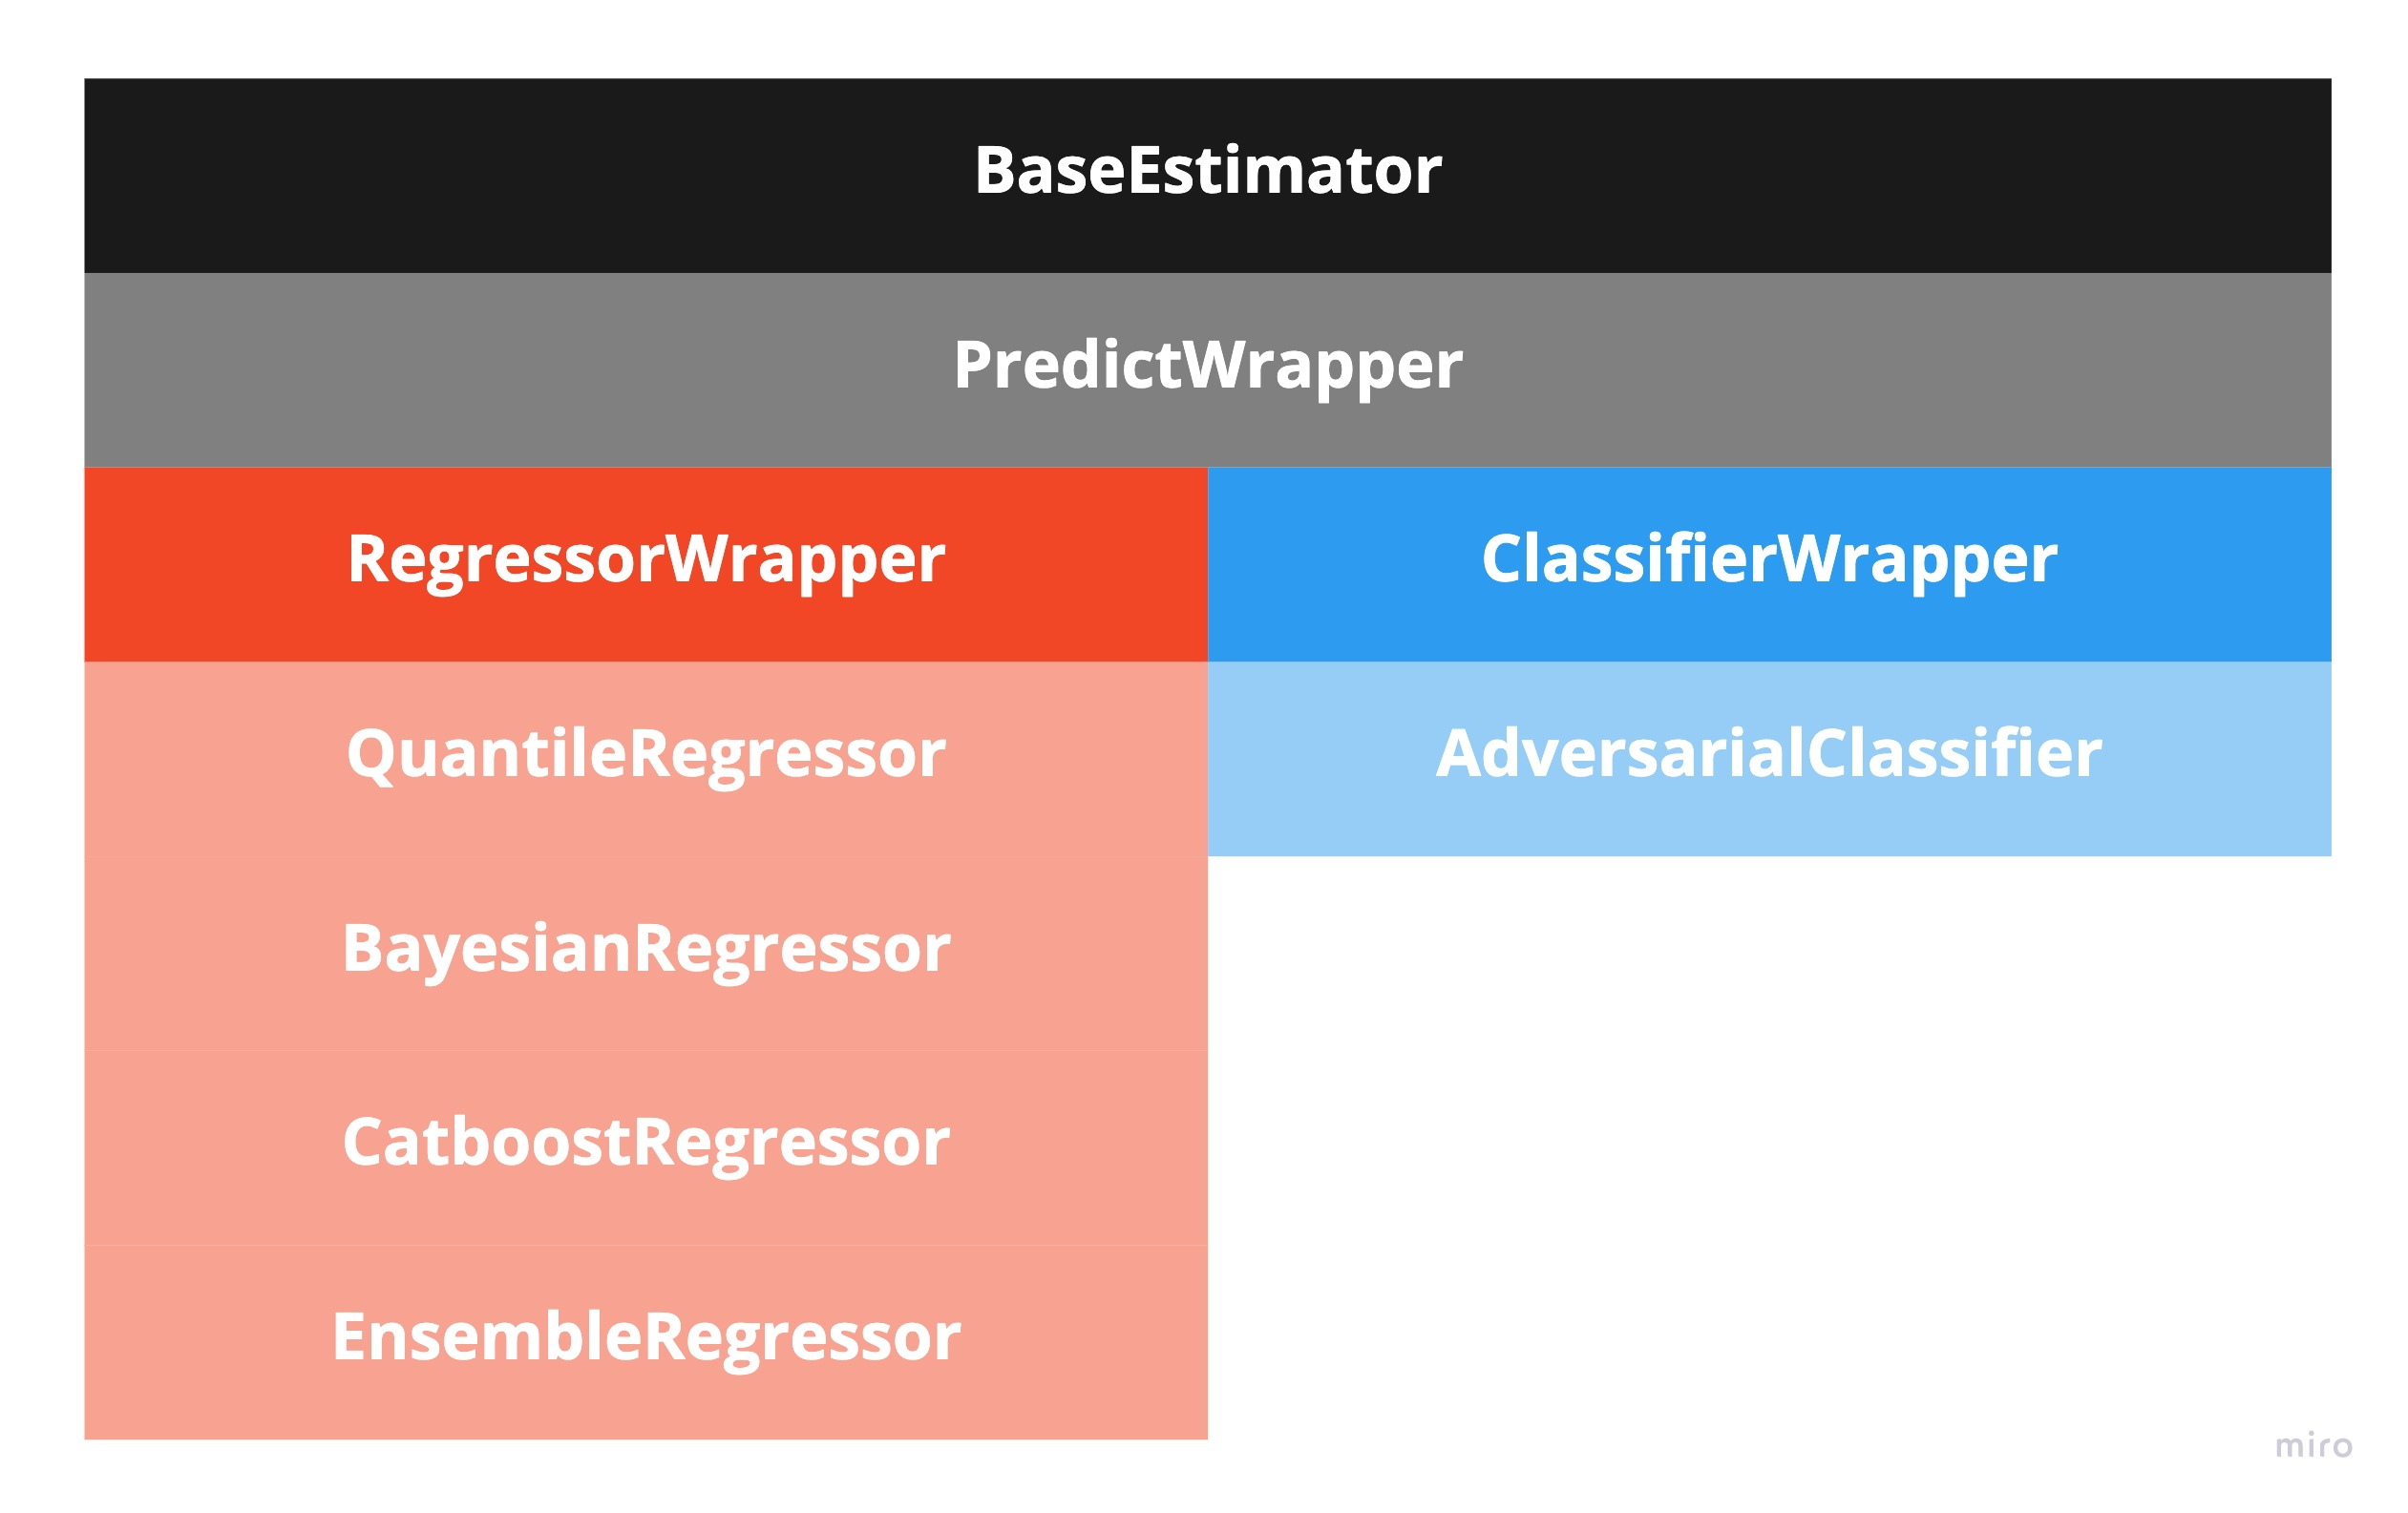
\includegraphics[width=1.15\textwidth]{figures/implementation/class-data-uq.jpg}
         \caption{Data UQ class wrappers.}
         \label{fig:data-uq-class}
     \end{subfigure}
     \hfill
     \begin{subfigure}[b]{0.32\textwidth}
         \centering
         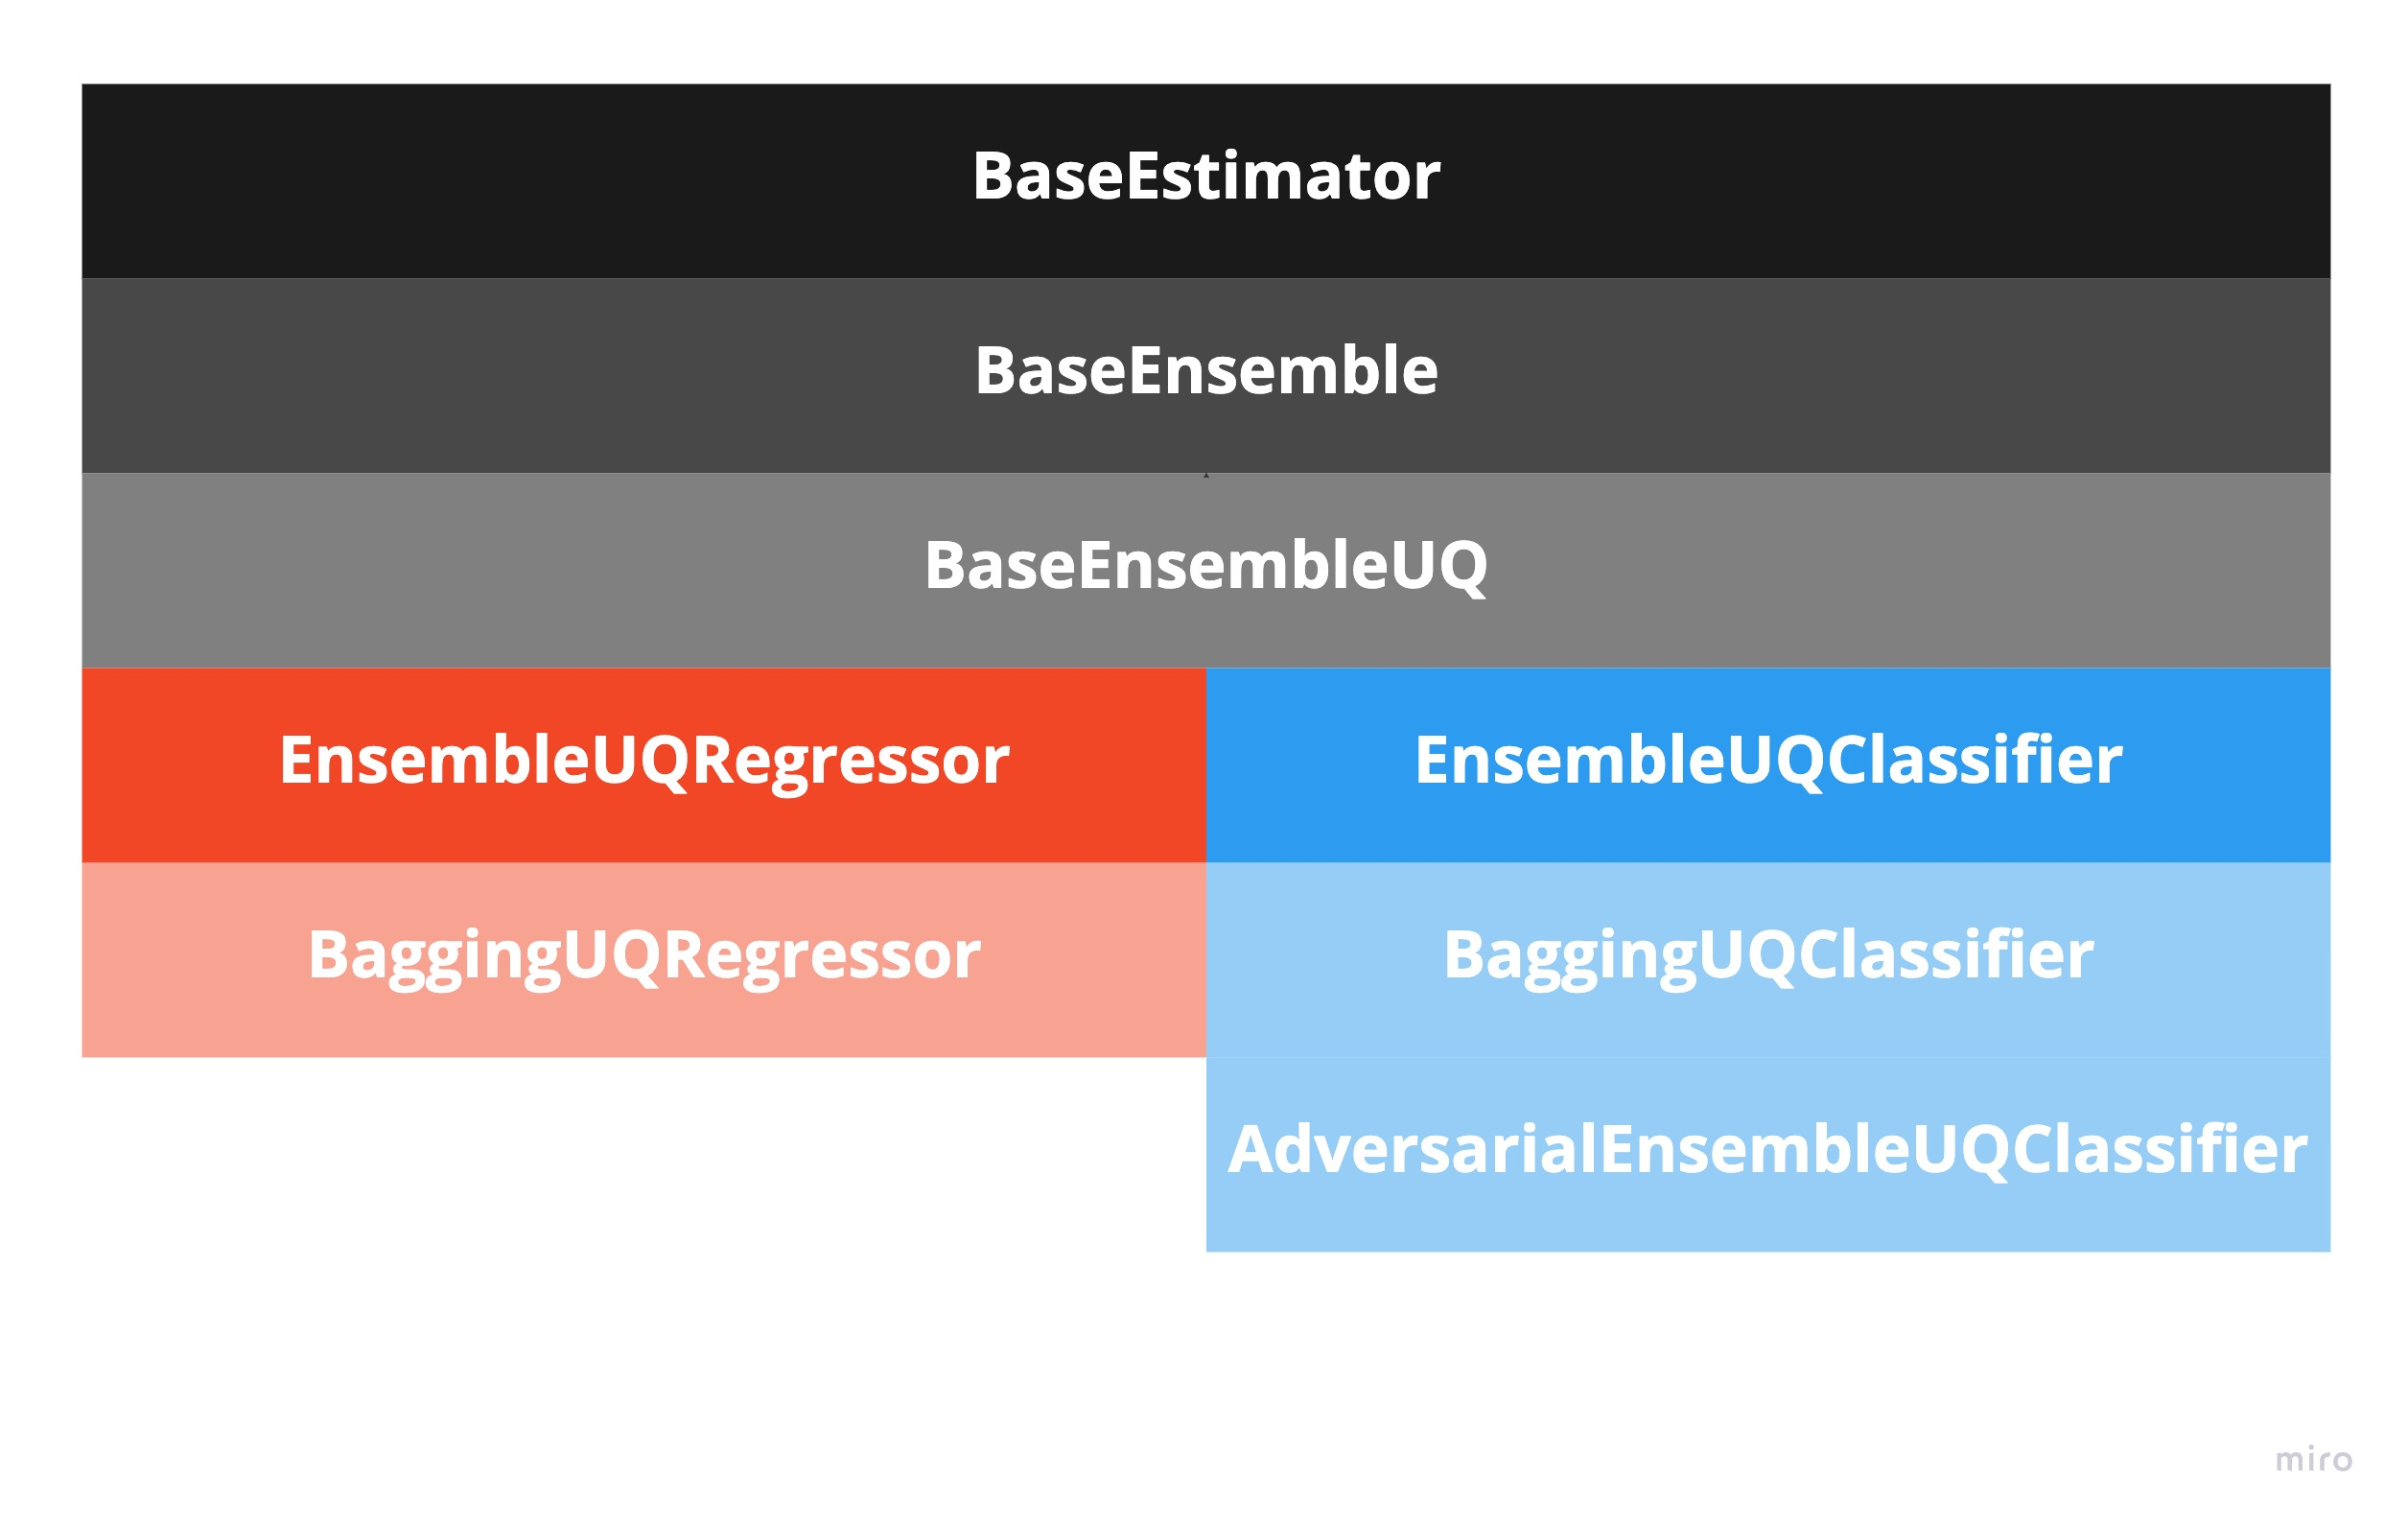
\includegraphics[width=1.15\textwidth]{figures/implementation/class-model-uq.jpg}
         \caption{Model UQ class wrappers.}
         \label{fig:model-uq-class}
     \end{subfigure}
     \hfill
     \begin{subfigure}[b]{0.32\textwidth}
         \centering
         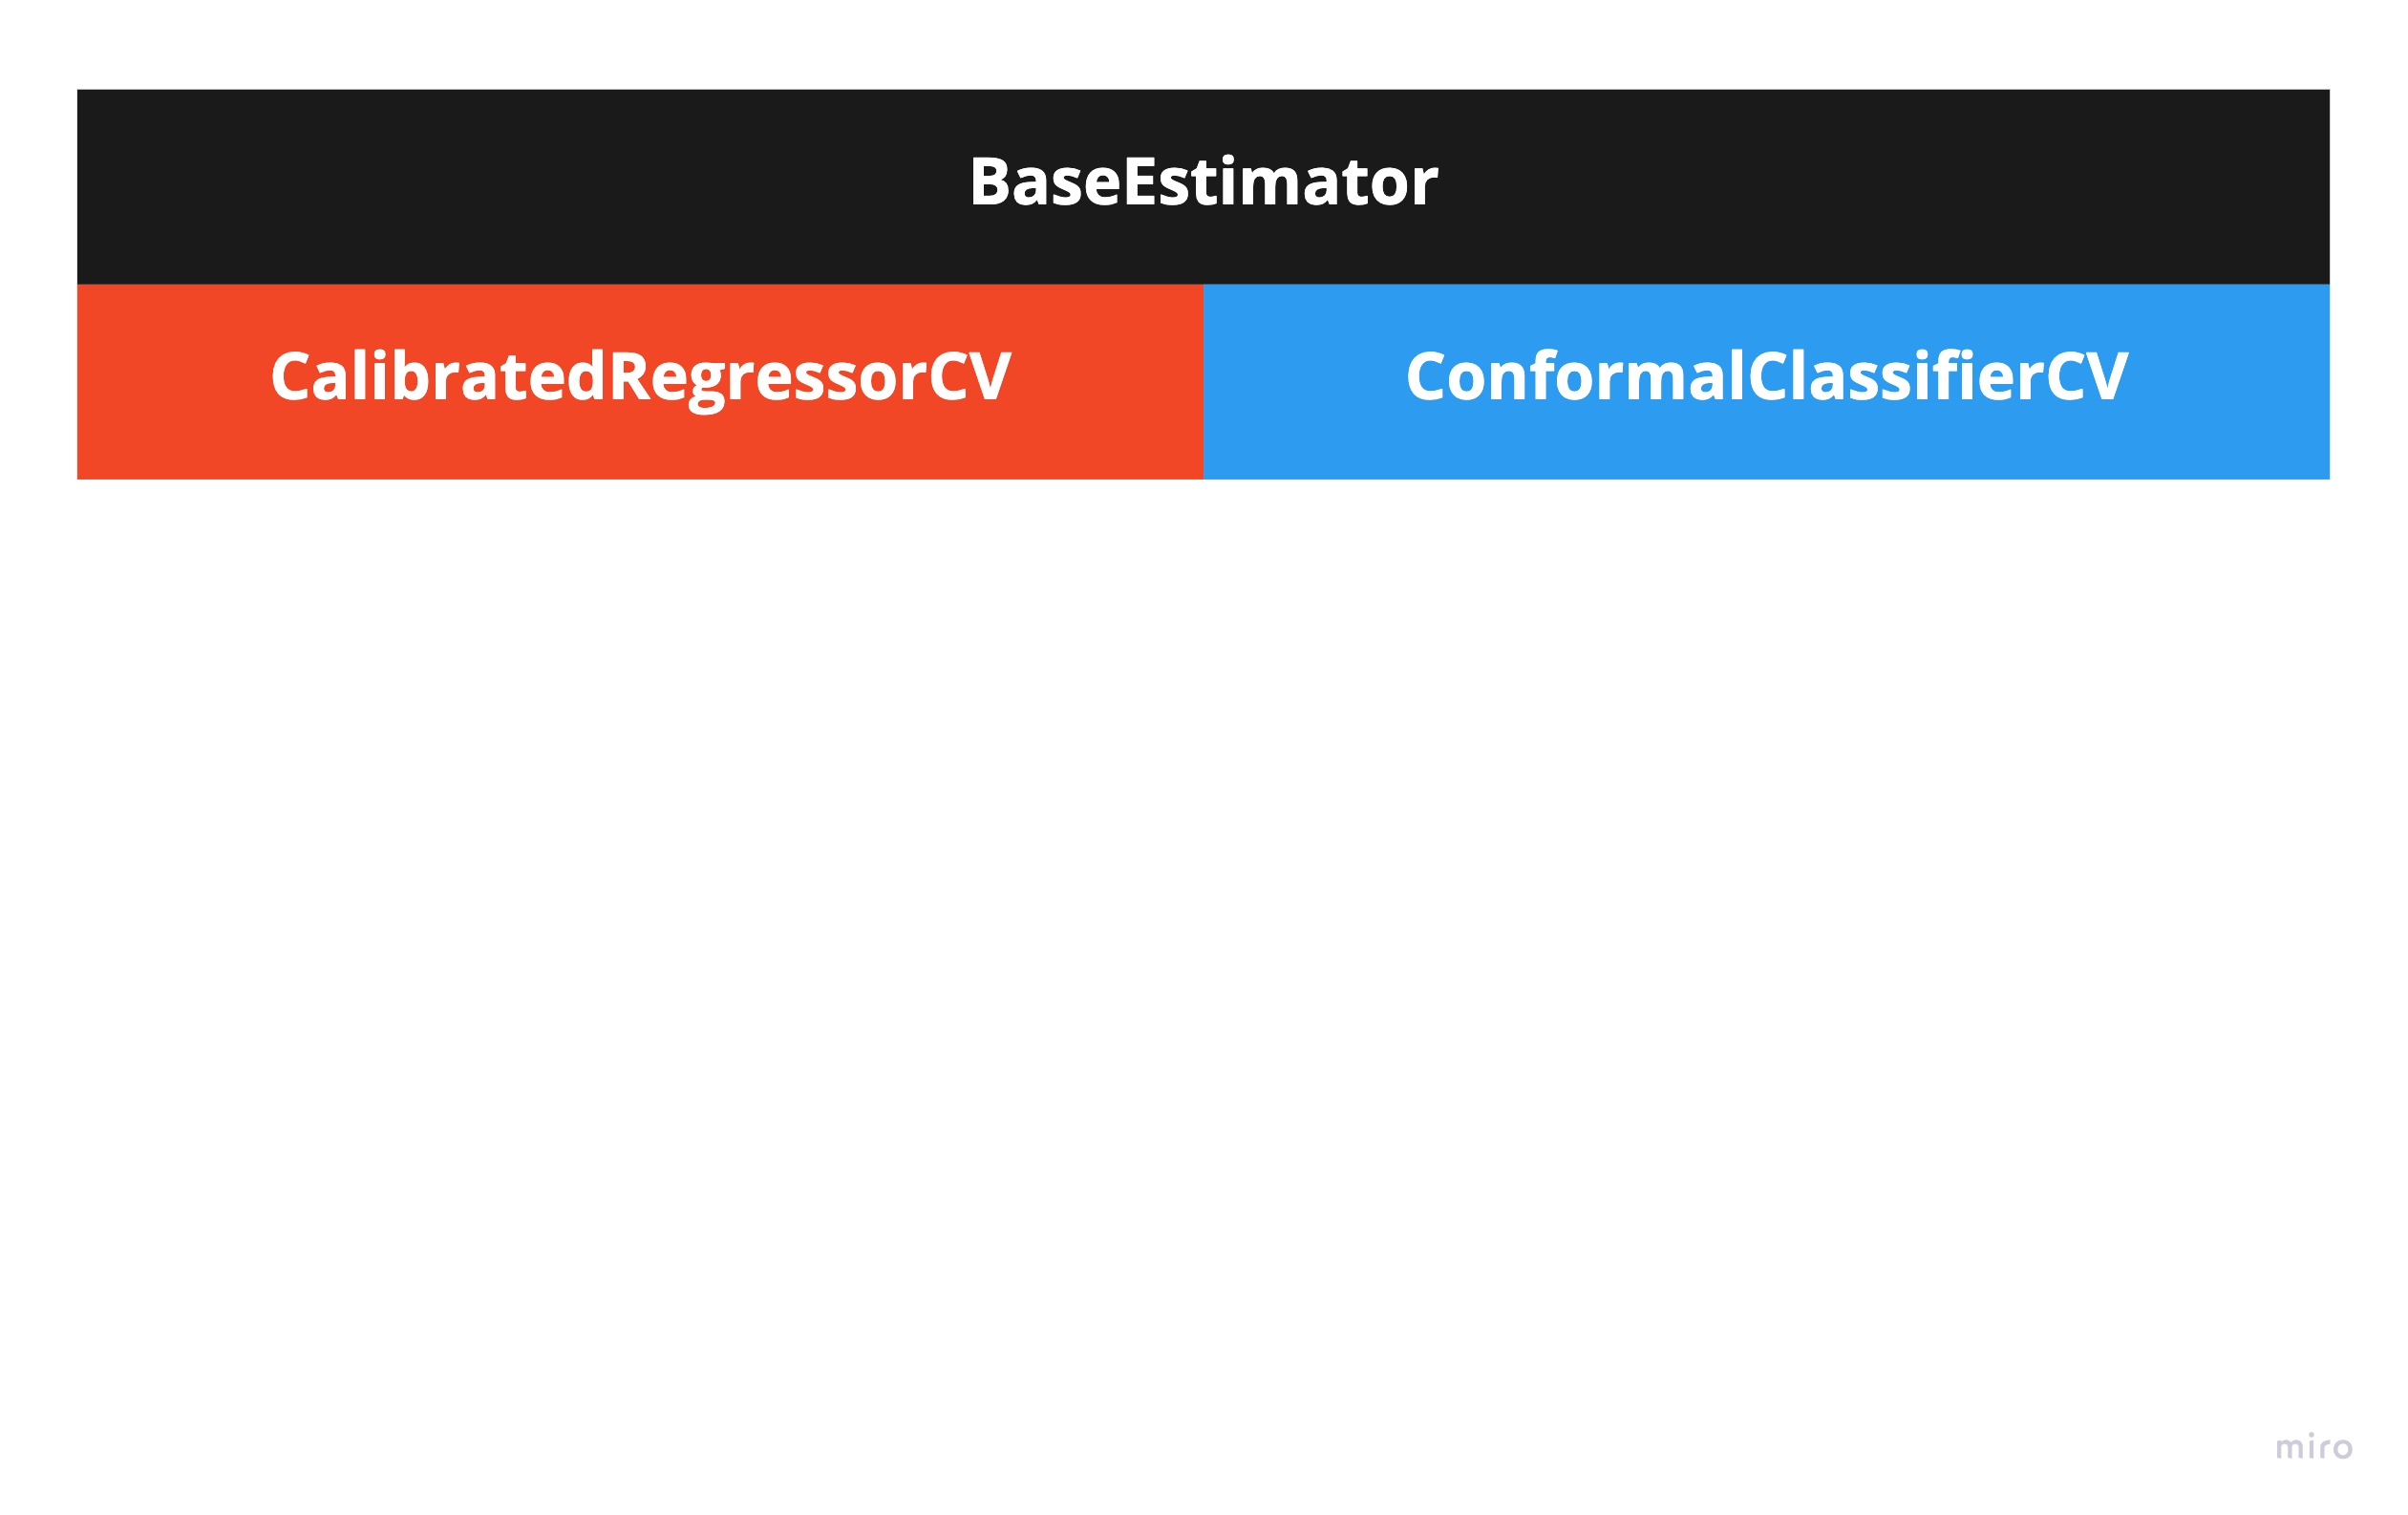
\includegraphics[width=1.15\textwidth]{figures/implementation/class-calibration.jpg}
         \caption{Calibration class wrappers.}
         \label{fig:calibration-uq-class}
     \end{subfigure}
        \caption{Class hierarchy of UQ package. Abstract classes are represented in grey and black. The first black level contains base classes from the \textit{scikit-learn} library. }
        \label{fig:class-hierarchy}
\end{figure}

% Overview of the scikit-learn package




\section{Open-source libraries}

Research and comparison of the different open-source uncertainty quantification tools have been carried out before the development of the package (cf. table \ref{fig:open-source-uq}). 
Most libraries are at a research/development level or are not maintained anymore and cannot be effectively used in production environments. %The Uncertainty Baselines gather metrics, datasets and UQ models for research use. 
We took a step toward simplicity of use and target \textit{scikit-learn} compatibility, which is not offered by any of these libraries except for \textit{Mapie}, \textit{CatBoost} and \textit{UQ360}. However, the first only covers distribution-free models for data UQ, while the second solely focuses on gradient-boosting models. On the other hand, \textit{UQ360} is probably the most similar tool to this work. However, one of our crucial selling points is that any \textit{scikit-learn} compatible model can be turned into a UQ model, which is not the case for \textit{UQ360}. Most of the meta-estimators of our package can exploit intrinsic attributes of models such as Random Forest or Gradient Boosted Trees to perform UQ without the need to provide a calibration dataset. Furthermore, \textit{UQ360} requires more prior uncertainty knowledge to develop UQ models and does not provide adversarial robustness evaluation nor conformal predictions. % unified API classification and regression.

Eventually, the final version of the package harnesses the benefits of these different tools to build a robust and standardised API, e.g. \textit{CatBoost}'s probabilistic learning and virtual ensemble capabilities, \textit{Mapie}'s quantile regression model and some metrics and plots of the \textit{uncertainty toolbox}. In addition, the \href{https://github.com/Trusted-AI/adversarial-robustness-toolbox}{Adversarial Robustness Toolbox (\textit{ART})} was used in the development, in particular their evasion attacks and adversarial training classes. Adversarial UQ wrappers available in the package are based on \textit{ART}. 

Finally, the inclusion of Bayesian learning methods into the package is discussed. After an exploration and testing phase of \textit{PyMC}, \textit{Edward2}, and \textit{PyMC-learn}, it was decided not to include them in this work. \textit{PyMC} and \textit{Edward2} are flexible approaches. Still, they often require manual tuning of prior model distributions and domain expertise to reach a model that is fast to train and accurate. It is, therefore, rather cumbersome to create a simple, \textit{scikit-learn}-like and unified API to train such models without going against the core principles of Bayesian learning. This was the initial objective of the \textit{PyMC-learn} project. However, it is currently left in an unmaintained state and is unusable given our requirements.

% pymc learn 

%- not been updated to the newest major release of PyMC (4.0) 
%Furthermore, as explained in the introductory section \ref{intro:motivation}, there is a clear lack of standardisatisation 



% presents an overview of existing open-source libraries for uncertainty quantification
% Pros and cons
% Why our package is needed.

\begin{table}[htbp]
\centering
\caption{Open-source uncertainty quantification libraries.}
\label{fig:open-source-uq}
\begin{tabular}[t]{p{2.6cm}p{1.4cm}p{1cm}p{1.8cm}p{3.3cm}p{1.5cm}p{2cm}} % 
\toprule
Name & Actor & GitHub stars & Latest release & Focus / Keywords & User friendly & Sk-learn compatible\\
\midrule
Uncertainty Toolbox (\href{https://github.com/uncertainty-toolbox/uncertainty-toolbox}{link}) &---& 1.3k &  Sep. 2021 & metrics, visualisation & high & no\\
Mapie (\href{https://github.com/scikit-learn-contrib/MAPIE}{link}) &---& 500 & Oct. 2022 & metrics, quantile regression, interval estimation  & high & yes\\
CatBoost (\href{https://github.com/catboost/catboost}{link})  &---& 6.9k & Nov. 2022 & gradient-boosted-trees & high & yes\\
UQ 360 (\href{https://github.com/IBM/UQ360}{link} ) & IBM & 176 & --- & General & medium & yes \\
Uncertainty baselines (\href{https://github.com/google/uncertainty-baselines}{link}) & Google & 1k & --- & DL research & low & no\\ 
PyMC (\href{https://github.com/pymc-devs/pymc}{link}) &---& 7.2k & Dec. 2022 & Bayesian learning & low & no\\
Edward2 (\href{https://github.com/google/edward2}{link}) & Google & 619 & --- & Bayesian learning, DL, TensorFlow & low & no\\
PyMC-learn (\href{https://github.com/pymc-learn/pymc-learn}{link}) & --- & 200 & Not maintained & PyMC, sk-learn & high & yes \\
\bottomrule
\end{tabular}
\end{table}%